%%%%%%%%%%%%%%%%%%%%%%%%%%%%%%%%%%%%%%%%%%%%%%%%%%%%%%%%%%%%%%%%%%%%%%%%%%%%%%%
% ICML 2025 SUBMISSION DRAFT: Event-based Tactile Pole Balancing
%%%%%%%%%%%%%%%%%%%%%%%%%%%%%%%%%%%%%%%%%%%%%%%%%%%%%%%%%%%%%%%%%%%%%%%%%%%%%%%

\documentclass{article}

% Recommended, but optional, packages for figures and better typesetting:
\usepackage{microtype}
\usepackage{graphicx}
\usepackage{subcaption}
\usepackage{booktabs} % for professional tables
\usepackage{hyperref}
\usepackage{booktabs}
% Attempt to make hyperref and algorithmic work together better:
\newcommand{\theHalgorithm}{\arabic{algorithm}}

% Use the following line for the initial blind version submitted for review:
% \usepackage{icml2025}
% If accepted, instead use the following line for the camera-ready submission:
\usepackage[accepted]{icml2025} % using [accepted] to show author names in draft

% For theorems and such
\usepackage{amsmath}
\usepackage{amssymb}
\usepackage{mathtools}
\usepackage{amsthm}

% if you use cleveref..
\usepackage[capitalize,noabbrev]{cleveref}

\icmltitlerunning{Learning Pole Balancing via Event-based Tactile Early Fusion}

\begin{document}

\twocolumn[
\icmltitle{Learning Pole Balancing via Event-based Tactile Early Fusion: \\
           A Comparative Analysis of Angular and Vectorial Representations}

\icmlsetsymbol{equal}{*}

\begin{icmlauthorlist}
\icmlauthor{Victor Pedreira Santos Pepe}{equal,tud,usp}
\icmlauthor{Thiago Daquino Velasquez}{equal,tud,usp}
\icmlauthor{Bárbara Fernandes Dias Bueno}{equal,tud,usp}
\icmlauthor{Tim Schneider}{tud}
\icmlauthor{Niklas Funk}{tud}
\end{icmlauthorlist}

\icmlaffiliation{tud}{Department of Electrical Engineering and Information Technology, TU Darmstadt, Darmstadt, Germany}
\icmlaffiliation{usp}{Polytechnic School, University of São Paulo (Poli-USP), São Paulo, Brazil}

\icmlcorrespondingauthor{Victor Pedreira Santos Pepe}{victor.pepe@stud.tu-darmstadt.de}
\icmlcorrespondingauthor{Thiago Daquino Velasquez}{thiago.velasquez@stud.tu-darmstadt.de}
\icmlcorrespondingauthor{Bárbara Fernandes Dias Bueno}{barbara.bueno@stud.tu-darmstadt.de}

\icmlkeywords{Machine Learning, ICML, Tactile Sensing, Event-based Vision, Robotics, Deep Learning, Pole Balancing}

\vskip 0.3in
]

\printAffiliationsAndNotice{\icmlEqualContribution} 

\begin{abstract}
    Precise estimation of object orientation from tactile feedback is critical for robotic manipulation, particularly in scenarios where visual sensing is unreliable or unavailable. We study 3D pole orientation estimation from high-resolution tactile time-series data, motivated by tactile-based pole balancing, and formulate the problem as regression on the unit sphere $S^2$. Direct learning from raw tactile pressure maps is challenged by high dimensionality and spatial redundancy, which we address through a Statistical Multi-Quad encoding that aggregates activations into structured spatial-statistical features at multiple resolutions. Ground-truth orientation vectors are computed from optical marker data via Singular Value Decomposition (SVD), and evaluation employs strict temporal splits across recording sessions to prevent interpolation-induced leakage. We compare memoryless, short-term temporal, and long-horizon sequence models under multiple target parameterizations. Our results show that the \textbf{statistical based TCN} model achieves the mean angular error of approximately \textbf{2.23°} on validation data, highlighting the importance of structured tactile representations combined with temporal modeling for accurate and stable orientation regression.
    \end{abstract}

    \section{Introduction}
    \label{intro}
    
    Reliable estimation of object orientation is a fundamental requirement in robotic manipulation, particularly in contact-rich tasks where visual sensing is occluded or unreliable. While vision-based pose estimation has matured significantly, tactile sensing remains comparatively underexplored as a primary modality for high-precision orientation inference. Tactile signals inherently encode rich spatial and temporal information about contact geometry, force distribution, and object dynamics. Leveraging these signals for accurate orientation estimation is essential for tasks such as pole balancing, where small angular deviations critically affect stability.
    
    Despite recent advances in high-resolution tactile sensors, learning directly from raw tactile pressure maps presents significant challenges. The dimensionality of modern tactile arrays is high, spatial activations are redundant, and contact patterns evolve over time in structured but non-trivial ways. Naively applying deep models to flattened tactile matrices risks overparameterization, inefficient learning, and poor generalization. Moreover, improper train-test splitting in time-series tactile data can introduce interpolation-induced leakage, leading to overestimated performance.
    
    Previous work in tactile sensing has mostly focused on classification tasks such as slip detection, using either end-to-end convolutional models or handcrafted features. Few studies have systematically explored the combination of spatially structured aggregation with both non-temporal and temporal modeling for accurate 3D orientation regression. Because orientation lies on the unit sphere, both feature representations and evaluation metrics must respect the geometric structure of rotations. Our work addresses this gap by evaluating memoryless feature-based models, short-horizon temporal models, and long-horizon sequence models under a unified statistical encoding framework.
    
    This raises a natural question:
    
    \textbf{How can high-dimensional tactile signals be represented and learned to enable accurate and stable 3D orientation regression under strict temporal generalization?}
    
    To answer this question, we introduce a Statistical Multi-Quad encoding that aggregates tactile activations into structured spatial-statistical features at multiple resolutions, reducing dimensionality while preserving geometric information. Ground-truth orientation vectors are derived via Singular Value Decomposition (SVD) from optical marker data, and evaluation is conducted using temporally disjoint recording sessions to prevent data leakage.
    
    Our key contributions are summarized as follows:

    \begin{enumerate}
        \item We formalize tactile-based pole orientation estimation as a regression problem on the unit sphere, enabling geometrically consistent evaluation through angular error metrics.
        
        \item We introduce a Statistical Multi-Quad encoding that aggregates tactile activations into spatial-statistical features at multiple resolutions, providing an efficient representation of high-dimensional tactile signals.
        
        \item We perform a systematic comparison of memoryless and temporal neural architectures for tactile orientation regression under temporally disjoint evaluation protocols.
    \end{enumerate}


    \section{Background}

    \subsection{Event-Based Optical Tactile Sensing}
    
    Optical tactile sensors measure contact by observing the deformation of a compliant elastomer through an internal camera. In contrast to RGB-based designs, event-based optical tactile sensors use neuromorphic cameras that asynchronously report pixel-level intensity changes. The EvETac sensor replaces a standard frame-based camera with an event-based camera, enabling high temporal resolution while maintaining fine spatial detail. Marker tracking algorithms reconstruct elastomer deformation from sparse event streams at rates up to 1000 Hz.
    
    In this design, tactile measurements resemble images defined over the sensor surface. Each contact produces a spatial activation pattern corresponding to local pressure and shear forces. Consequently, a single tactile snapshot consists of hundreds of spatially distributed measurements, yielding high-dimensional signals. Over time, these spatial patterns evolve according to object motion and contact dynamics, forming structured tactile time-series data.
    
    \subsection{Sparse Polarity-Based Tactile Signals}

    Each tactile measurement is represented as a spatial map whose entries take values in $\{-1, 0, +1\}$, corresponding to negative events, no change, and positive events, respectively. Due to the event-based sensing mechanism, the majority of entries are zero at any given time step, yielding highly sparse activation patterns.
    
    Positive and negative events encode distinct local deformation dynamics of the elastomer surface. Consequently, the tactile signal forms a sparse signed spatial field rather than a dense pressure image. Directly flattening this representation leads to high-dimensional vectors dominated by zeros and ignores meaningful spatial organization.
    
    To extract informative structure while reducing dimensionality, spatial events can be aggregated into statistical descriptors. Computing quantities such as centroids, spatial dispersion, and event counts—either jointly or separately for positive and negative activations—provides a compact summary of contact geometry while preserving polarity-specific information.
     
    \subsection{Orientation Representation on the Unit Sphere}
    
    We represent pole orientation as a 3D unit vector $\mathbf{v} \in \mathbb{R}^3$ satisfying $\|\mathbf{v}\|_2 = 1$. The set of all such vectors defines the unit sphere $S^2$. Formulating orientation estimation as regression on $S^2$ ensures a continuous and non-redundant representation, avoiding discontinuities inherent in Euler angles.
    
    Given a predicted vector $\hat{\mathbf{v}}$ and ground truth $\mathbf{v}$, performance is evaluated using angular error:
    \[
    \theta = \arccos \left( \hat{\mathbf{v}}^\top \mathbf{v} \right).
    \]
    
    This metric directly measures rotational discrepancy in degrees and respects the geometry of the sphere.

    \section{Related Work}

    \subsection{Event-Based Tactile Sensing}
    
    Recent work introduced event-based optical tactile sensors to overcome the temporal limitations of frame-based designs. The EvETac sensor demonstrated high-frequency deformation tracking and efficient slip detection using sparse asynchronous event streams. While these works establish the hardware capabilities of event-driven tactile sensing, they primarily focus on contact classification and force reconstruction rather than continuous geometric state regression.
    
    \subsection{Tactile Pose Estimation}
    
    Tactile pose estimation has been studied in both object-specific and category-level settings. Tac2Pose proposes an object-specific framework that estimates object pose from the first tactile contact by matching observed contact shapes against simulated ones. This approach relies on known object geometry and large-scale simulation to learn pose-conditioned embeddings.
    
    Kelestemur et al.\ investigate category-level tactile pose estimation using a Bayesian filtering framework with a learned tactile observation model. Their method integrates simulation-based training and reinforcement learning for downstream manipulation tasks.
    
    In contrast to these approaches, our work does not assume access to object meshes, precomputed contact simulations, or filtering frameworks. Instead, we focus on direct regression of 3D orientation from sparse event-based tactile signals collected exclusively in the real world.
    
    \subsection{Learning Architectures for Tactile Signals}
    
    Learning-based tactile perception methods typically employ either handcrafted features or end-to-end convolutional models operating on dense tactile images. Temporal architectures such as LSTMs have been applied for slip detection and dynamic contact modeling. However, systematic comparisons between memoryless and temporal architectures for high-frequency geometric regression under temporally disjoint evaluation protocols remain limited. Our work isolates the effects of structured spatial encoding and sequence modeling for orientation regression under strict temporal generalization.
    
\section{Methodology}
\subsection{Problem Formulation}
The ultimate objective of this work is to balance a pole using exclusively tactile sensing.
More specifically, we aim to estimate the pole orientation relying only on the robot state
information and the tactile sensor events, without using visual input during inference.

At each time step, the system has access to: (i) the robot state variables
(e.g., position and orientation of the sensor support),
and (ii) the sparse event-based tactile measurements provided by the tactile sensor.
Based on these inputs, the goal is to predict the 3D orientation of the pole.

Formally, let $\mathbf{x}_t$ denote the robot state at time $t$,
and let $\mathbf{s}_t$ represent the corresponding tactile sensor measurements.
The task is to learn a function
\[
f_\theta : (\mathbf{x}_{t-k:t}, \mathbf{s}_{t-k:t}) \rightarrow \mathbf{y}_t,
\]
where $\mathbf{y}_t$ denotes the pole orientation at time $t$,
$\theta$ represents the learnable model parameters,
and $k$ defines the size of the temporal window used as input.

To address this problem, we train and evaluate multiple deep learning models
for pole orientation prediction. Their performance is systematically compared
and optimized with the objective of achieving sufficient accuracy to support
stable closed-loop control.

\subsection{Data Collection}
We opted to collect real human data to train the proposed model in order to capture realistic interaction dynamics,
sensor noise, and natural variability, that would not be able to be fully replicated in a simulated environment.
The human data collection also proved to be better for capturing more extreme pole angles, differently from a robotic setup where the pole would likely fall after reaching such angles.

For that pourpose, we designed a custom support equipped with an \textit{Evtac} tactile sensor, and a set of \textit{OptiTrack} markers.
This support was used by human operators, to perform the balancing task, while the tactile and motion capture data were recorded simultaneously.

Ground-truth measurements of the pole angle together with support angle and position were obtained using an \textit{OptiTrack} motion capture system, which provides accurate 3D pose estimation.
The motion capture data was temporally synchronized with the tactile sensor readings to ensure alignment between input signals and target labels.

Aiming to obtain a more varied dataset, we recorded multiple sessions with two different team members.
Also, to ensure a fair and unbiased evaluation, one complete recording from each member were reserved exclusively for testing.
This recordings were not used during training or validation. The remaining data was split into training and validation sets.
All evaluated models were trained and validated using exactly the same data to guarantee a consistent comparison.

\begin{figure}[htbp]
    \centering
    
    \begin{subfigure}{0.48\linewidth}
        \centering
        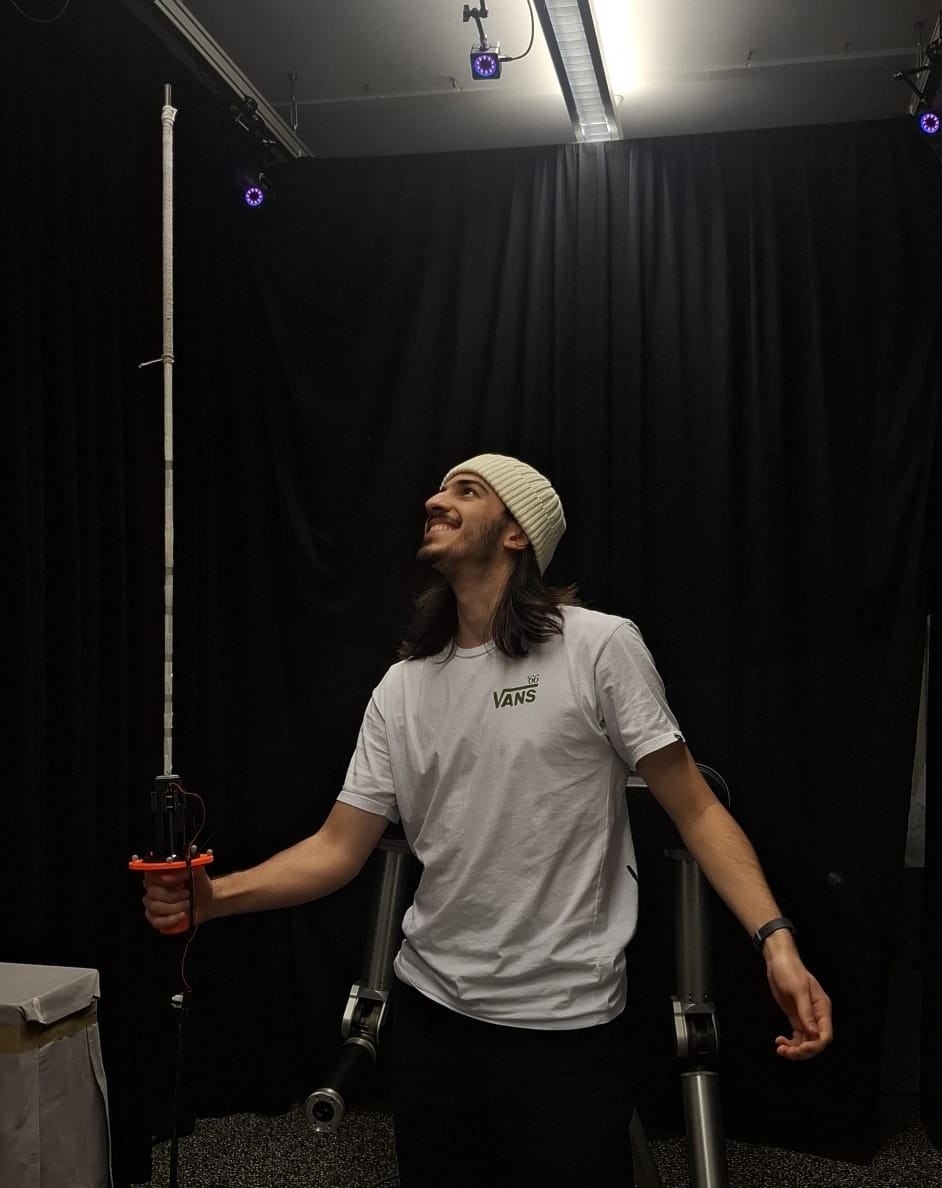
\includegraphics[width=\linewidth]{images/thiago_balancing.jpeg}
        \caption{One of the team members performing the pole balancing task.}
        \label{fig:img1}
    \end{subfigure}
    \hfill
    \begin{subfigure}{0.48\linewidth}
        \centering
        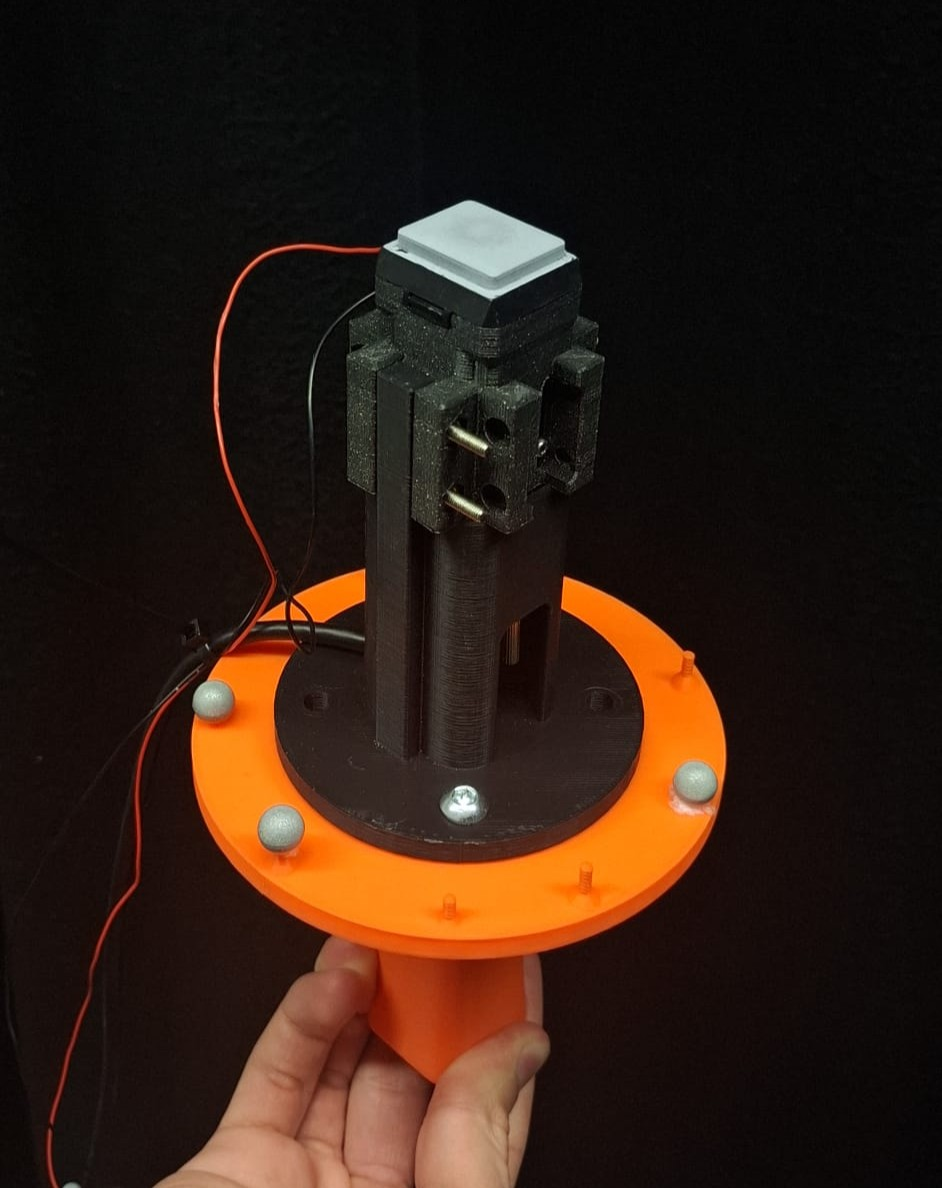
\includegraphics[width=\linewidth]{images/holder.jpeg}
        \caption{Personalized support equipped with an \textit{Evtac} tactile sensor and \textit{OptiTrack} markers.}
        \label{fig:img2}
    \end{subfigure}
    
    \caption{Human data collection setup.}
    \label{fig:comparison}
\end{figure}

\subsection{Metrics}
\subsubsection{Loss Function}

Pole orientation is represented as a unit vector $\mathbf{v} \in S^2$.
Given a predicted vector $\hat{\mathbf{v}}$ and the corresponding ground-truth
vector $\mathbf{v}$, both normalized to unit length, we train the models
using an angular regression loss defined as

\begin{equation}
\mathcal{L}_{\text{ang}} =
\arccos
\left(
\operatorname{clamp}
(\hat{\mathbf{v}} \cdot \mathbf{v}, -1, 1)
\right).
\end{equation}

This loss corresponds to the geodesic distance between the predicted
and ground-truth orientations on the unit sphere $S^2$. Compared to
Euclidean losses on vector components, the angular loss directly
penalizes rotational deviation and therefore aligns with the geometric
structure of the orientation estimation task.

The predicted vectors are normalized before computing the loss to
ensure that both predictions and targets lie on the unit sphere.

\subsection{Arquitectures and Approaches}
\subsubsection{Multi Layer Perception Network (MLP)}
We employ a Multilayer Perceptron (MLP) as an initial baseline to map spatial tactile features directly to the pole's 3D orientation vector. This instantaneous mapping provides a rapid evaluation of the sensor's representational power prior to modeling complex temporal dynamics.

The architecture utilizes a progressive bottleneck with five hidden layers (128, 256, 128, 64, and 32 neurons). To ensure stable gradients and mitigate overfitting on sparse data, each linear transformation is followed by 1D Batch Normalization, ReLU activation, and a Dropout layer (rate of 0.1).

% Multilayer Perceptrons  are foundational feedforward neural networks consisting of fully connected layers, effective at approximating complex, non-linear mappings. In this study, an MLP was employed as an initial baseline model due to its architectural simplicity and exceptionally fast training and inference speeds. By treating the pole balancing task initially as an instantaneous mapping---from spatial tactile features directly to the pole's orientation vector---the MLP provided a rapid evaluation of the sensor's base representational power before introducing more complex temporal dynamics.
%
% The implemented architecture, \textit{TactileMLPVector}, utilizes a progressive bottleneck structure to compress the input features into a 3D directional vector. The network consists of five hidden layers with 128, 256, 128, 64, and 32 neurons, respectively. To ensure stable gradient propagation and mitigate overfitting on the sparse tactile data, each linear transformation is followed by 1D Batch Normalization, a Rectified Linear Unit (ReLU) activation function, and a Dropout layer with a rate of 0.1.
% Multilayer Perceptrons (MLPs) are foundational feedforward artificial neural networks widely used for structured data processing and regression tasks. Unlike specialized architectures such as convolutional or recurrent networks, MLPs consist entirely of fully connected layers, where each neuron in a given layer connects to all neurons in the subsequent layer. Through the use of non-linear activation functions, MLPs are capable of approximating complex, high-dimensional mappings. Due to their architectural simplicity, deterministic execution, and highly optimized matrix multiplication operations, MLPs provide exceptionally fast training and inference times, making them an ideal choice for rapid prototyping and establishing strong empirical baselines.
\subsubsection{Convolutional Neural Network (CNN)}
Convolutional Neural Networks (CNNs) are specialized deep learning architectures designed to process grid-like data using localized filters. For tactile-based pole balancing, CNNs offer an intuitive approach by directly operating on the accumulated 2D pixel matrix of the EveTac sensor. By applying sliding learnable kernels across multiple channels, the network can extract a rich hierarchy of spatial features—ranging from basic edges to complex contact geometries. This enables the model to natively learn the spatial morphology and intensity distributions of the pole's footprint, bypassing the need for hand-crafted statistical feature extraction.

However, this direct processing of dense spatial matrices introduces significant trade-offs. The architectural complexity and the high volume of floating-point operations drastically elevate both training and inference times compared to lightweight MLP baselines. While CNNs can capture fine spatial nuances, their heavy computational burden presents practical challenges for high-frequency, real-time control applications.
\subsubsection{Temporal Convolutional Network (TCN)}
Temporal Convolutional Networks (TCNs) are convolutional architectures
designed for sequence modeling tasks. Unlike recurrent neural networks, TCNs rely
exclusively on one-dimensional causal convolutions applied along the temporal dimension,
ensuring that predictions at time $t$ depend only on current and past inputs.
To effectively capture long-range temporal dependencies, TCNs employ dilated convolutions,
where the dilation factor increases exponentially with network depth, allowing the
receptive field to grow without a proportional increase in parameters.
Due to their parallelizable structure, stable gradients, and
flexible receptive field control, TCNs have shown competitive or superior performance
compared to recurrent models in various sequence modeling tasks \cite{bai2018empirical}.

In the context of tactile-based pole angle estimation, the use of a TCN
is well-motivated. Pole balancing is inherently
a dynamic problem, in which the current orientation depends on the recent temporal
evolution of contact patterns rather than on instantaneous measurements alone.
Since the tactile sensor operates in an event-based manner,
producing sparse and temporally structured signals,
modeling short- and long-term temporal dependencies is essential.
The causal structure of TCNs ensures that predictions rely only on past and
present information, making them suitable for real-time control scenarios.
Furthermore, dilated convolutions allow the network to aggregate information
over multiple temporal scales, which is beneficial for capturing both fast
transient contact events and slower motion trends of the pole.
Compared to recurrent architectures, TCNs also offer more stable training
and parallelizable computation, which is advantageous when training on long
tactile sequences.

The implemented TCN architecture was based on the design proposed by Bai et al. (2018) \cite{bai2018empirical},

\subsubsection{Statistical Feature Extraction Approach}

Processing raw, high-resolution tactile event streams directly imposes significant computational overhead. However, recent research on event-based tactile skins demonstrates that such data is highly compressible \cite{koolani2026event}. For instance, using stochastic down-sampling, an event stream could be reduced to $1/1024$ of its original size while maintaining valid press localizations for 85\% of the trials. Motivated by this inherent sparsity, we developed a spatial statistical feature extraction strategy to provide a fixed-size, lower-dimensional input representation for our models without losing essential mechanical information.

\par Rather than processing the full asynchronous event stream, our approach aggregates tactile data over discretized spatial regions to capture the macroscopic dynamics of the pole's contact footprint. The sensor's spatial domain is subdivided into a grid of independent, uniformly sized quadrants. The dimensions of these quadrants act as a crucial hyperparameter that balances spatial granularity against computational performance. Smaller quadrants provide high-resolution localization of tactile stimuli but exponentially increase the dimensionality of the feature vector, while larger quadrants yield a more compact representation at the cost of fine-grained spatial details.

\par Within each quadrant, the accumulated event stream is strictly segregated by polarity into positive events (typically indicating an increase in pressure) and negative events (indicating a decrease or release). For each processed frame, the algorithm extracts a set of foundational spatial statistics per quadrant: the mean spatial coordinates $(x, y)$, the spatial variance of the active pixels, and the absolute count of positive and negative events.

\par To further encode the geometric structure and distribution of the contact patches, the algorithm computes the seven Hu moments for the events within each quadrant. Hu moments are a well-established set of statistical descriptors invariant to image translation, scale, and rotation. They are calculated independently for both the positive and negative event masks to distinctly capture the dynamics of contact onset and release. To ensure numerical stability, a logarithmic transformation is applied to the raw moments via $-\text{sign}(h) \cdot \log_{10}(|h| + 10^{-7})$. This combination of basic spatial statistics and invariant shape descriptors provides a dense, information-rich vector that efficiently summarizes the tactile state at any given instantaneous timestep.

\subsubsection{Temporal Sliding Window Formulation}

While instantaneous spatial features are sufficient for memoryless baselines, pole balancing is inherently a dynamic system where the current orientation heavily relies on past trajectories. To explicitly capture this temporal evolution without altering the underlying spatial encoding, we extend the instantaneous tactile representations into the temporal domain using a sliding window formulation.

\par Let $X_t$ represent the extracted tactile features (e.g., the statistical vector) and base kinematic inputs at a discrete timestep $t$. A sliding window of size $T$ aggregates these past and current observations into a continuous sequence $S_t = \{X_{t-T+1}, \dots, X_{t-1}, X_t\}$. The sequential models are then trained to map this input history $S_t$ to the target pole orientation at the final timestep $t$. 

\par A stride parameter controls the step size of the sliding window across the dataset, determining the overlap between consecutive sequences. This formulation ensures that temporal architectures, such as the TCN, receive a consistent historical context. By framing the input this way, the models are forced to implicitly learn the velocity and acceleration trends of the pole's contact footprint across the sensor surface over time.


% \subsubsection{Statistical Feature Extraction Approach}
%
% Processing raw, high-resolution tactile event streams directly imposes significant computational overhead. However, recent research on event-based tactile skins demonstrates that such data is highly compressible \cite{koolani2026event}. For instance, using stochastic down-sampling, an event stream could be reduced to $1/1024$ of its original size while maintaining valid press localizations for 85\% of the trials . These results show that the sensing approach remains functional even with very sparse event data, which is promising for reducing computational load. Motivated by this inherent sparsity, we developed a spatial statistical feature extraction strategy to provide a fixed-size, lower-dimensional input representation for our models without losing essential mechanical information.
%
% \par Rather than processing the full asynchronous event stream, our approach aggregates tactile data over discretized spatial regions to capture the macroscopic dynamics of the pole's contact footprint. The sensor's spatial domain is subdivided into a grid of independent, uniformly sized quadrants. The dimensions of these quadrants act as a crucial hyperparameter that balances spatial granularity against computational performance. Smaller quadrants provide high-resolution localization of tactile stimuli but exponentially increase the dimensionality of the feature vector, potentially leading to sparse or empty regions. Conversely, larger quadrants yield a more compact and computationally efficient representation, though at the cost of fine-grained spatial details.
% \par Within each quadrant, the event stream is strictly segregated by polarity into positive events (typically indicating an increase in pressure or contact area) and negative events (indicating a decrease or release). For a given temporal window, the algorithm extracts a set of foundational spatial statistics per quadrant, including the mean spatial coordinates $(x, y)$, the spatial variance of the active pixels, and the absolute count of positive and negative events.
%
% \par To further encode the geometric structure and distribution of the contact patches, the algorithm computes the seven Hu moments for the events within each quadrant. Hu moments are a well-established set of statistical image descriptors that quantify the shape characteristics of a distribution. They are particularly valuable because they are invariant to image translation, scale, and rotation, allowing the model to recognize consistent contact patterns regardless of their precise location within the quadrant.The Hu moments are calculated independently for both the positive and negative event masks to distinctly capture the dynamics of contact onset and release. Because raw Hu moments can span several orders of magnitude, a logarithmic transformation is applied to the results $(-\text{sign}(h) \cdot \log_{10}(|h| + 10^{-7}))$ to ensure numerical stability and facilitate neural network training. This combination of basic spatial statistics and invariant shape descriptors provides a dense, information-rich vector that efficiently summarizes the tactile state at any given timestep.
%

\section{Experiments}

This section evaluates how different tactile representations and temporal modeling strategies affect pole orientation estimation from event-based tactile data. We first establish simple reference baselines that quantify how well the task can be solved without tactile sensing or with trivial predictions. These experiments motivate the need for tactile-based learning models. We then perform a systematic comparison of representation and temporal modeling approaches.

\subsection{Task Simplification Experiments}

Before evaluating learning architectures, we conducted two controlled experiments designed to establish lower-bound baselines for the task. These experiments test whether pole orientation can be estimated from support motion alone and whether a constant upright prediction already achieves low error due to the pole being frequently near vertical.

\paragraph{Support-Only Baseline.}
In the first experiment, we evaluate whether the orientation of the support alone is sufficient to predict the pole orientation. The tactile input is removed, and a simple multilayer perceptron (MLP) is trained using only the orientation of the support that the human operator holds during the balancing task.

This experiment serves as a baseline to quantify how much information about the pole state can be inferred from the support motion alone. Because the pole can move relative to the support during balancing, the support orientation provides only indirect information about the pole orientation. The results therefore establish that relying solely on this signal leads to significantly larger prediction errors, motivating the use of tactile sensing to capture the contact dynamics between the pole and the sensor.

\paragraph{Vertical-Pole Baseline.}
In the second experiment, we evaluate a trivial baseline that always predicts the pole to be perfectly vertical. Since the goal of the task is to keep the pole balanced upright, the pole remains close to the vertical direction for much of the dataset. This raises the question of whether a constant prediction might already achieve low error.

To assess this, we compute the orientation error obtained when the predicted pole angles are fixed at $0^\circ$ for all samples. This baseline measures the error incurred by ignoring the dynamics of the pole entirely and assuming it remains perfectly upright. Comparing our learned models to this baseline allows us to verify that the proposed approach captures meaningful variations in pole orientation and achieves substantially lower error than this trivial assumption.

Together, these experiments establish reference baselines for the task and demonstrate that neither support motion nor a constant upright assumption is sufficient to accurately estimate the pole orientation. This motivates the use of tactile sensing together with learned representations for reliable pole state estimation.

\subsection{Statistical Representation of Event-Based Tactile Data}

The raw tactile input consists of event streams where each event has a polarity of $-1$, $0$, or $1$, with the majority of pixels being inactive ($0$). To reduce redundancy and exploit the sparse nature of the signal, we convert the event map into a structured statistical representation.

The tactile surface is partitioned into a grid of spatial quadrants, and statistics are computed for positive and negative events within each region. These statistics include the centroid, standard deviation, and event count. Some features combine both polarities, while others are computed separately for positive and negative events. This representation summarizes the spatial distribution of tactile activity while preserving polarity information.

To determine the appropriate spatial resolution, we evaluate multiple quadrant sizes: $1$, $0.5$, $0.25$, and $0.125$ of the sensor area. This experiment analyzes how feature granularity affects prediction accuracy and computational complexity. Based on these results, a quadrant size of $0.25$ is selected for subsequent experiments as a balance between spatial detail and robustness.

\subsection{Temporal Modeling}

To understand the role of temporal information in tactile state estimation, we evaluate models with different levels of temporal context.

\paragraph{Memoryless Models.}
Memoryless models operate on individual tactile frames without explicitly modeling temporal dependencies. These models evaluate whether instantaneous tactile geometry is sufficient for predicting pole orientation.

\paragraph{Short-Context Models.}
Short-context models incorporate limited temporal information through sliding window representations. We evaluate windows of size $3$ and $5$, allowing the model to observe recent tactile activity while maintaining low latency.

\paragraph{Long-Context Models.}
Long-context temporal models based on Temporal Convolutional Networks (TCNs) are used to capture extended temporal dependencies in the tactile event stream. Dilated convolutions allow the receptive field to grow exponentially, enabling the model to integrate information over longer time horizons.

\subsection{Model Architectures}

We evaluate several combinations of tactile representations and neural architectures:

\begin{itemize}
    \item \textbf{TCN + CNN:} A temporal convolutional network applied to convolutional features extracted from the tactile event map.
    \item \textbf{TCN + Statistical Representation:} A temporal convolutional network operating on the structured statistical features derived from the sparse event representation.
    \item \textbf{Sliding Window + Statistical Representation:} Short-context models using statistical features aggregated over temporal windows of size $3$ and $5$.
\end{itemize}


This comparison allows us to analyze how spatial representation and temporal modeling interact when predicting pole orientation from event-based tactile signals.
\section{Results}
\begin{table}[H]
\centering
\resizebox{\columnwidth}{!}{%
\begin{tabular}{ccc}
\hline
\textbf{Grid Shape} & \textbf{Val Error (°)} & \textbf{Val Loss ($10^{-3}$)} \\ \hline
8x8                 & 3.505 $\pm$ 3.587         & 0.604                         \\
4x4                 & 3.462 $\pm$ 3.189         & 0.811                         \\
2x2                 & 3.441 $\pm$ 3.117         & 0.951                         \\
1x1                 & 3.924 $\pm$ 3.168         & 1.4607                        \\
\end{tabular}%
}
\caption{Comparison between MLP models with statistical features of different grid sizes (without sliding window)}
\label{tab:mlp_grids}
\end{table}


% Please add the following required packages to your document preamble:
% \usepackage{booktabs}
% Please add the following required packages to your document preamble:
% \usepackage{booktabs}
\begin{table}[H]
\centering
\setlength{\tabcolsep}{4pt}
\renewcommand{\arraystretch}{0.92}
\resizebox{\columnwidth}{!}{%
\begin{tabular}{@{}ccc@{}}
\toprule
\textbf{Model} & \textbf{Val Error (°)} & \textbf{Val Loss ($10^{-3}$)} \\ \midrule
Vertical Pole Baseline           & 9.844 $\pm$ 4.277  & 10.645 \\
MLP Support Only                 & 5.232 $\pm$ 3.297  & 3.953 \\
MLP Stats (2x2)                  & 3.441 $\pm$ 3.117  & 0.951 \\
MLP Sliding Window + Stats (2x2) & 3.126 $\pm$ 3.0458 & 0.553 \\
TCN+Stats (2x2)                  & 2.229 $\pm$ 2.921  & 0.016 \\
CNN+TCN                          & 3.613 $\pm$ 3.464  & 0.350 

\end{tabular}%
}
\caption{Comparison between all models}
\label{tab:best_models}
\end{table}
\setlength{\tabcolsep}{6pt}
\renewcommand{\arraystretch}{1}
% \begin{table}[H]
% \begin{tabular}{@{}cccc@{}}
% \toprule
% \textbf{Model}                   & \textbf{Val Error (°)} & \textbf{Val Error Std. (°)} & \textbf{Val Loss (10\textasciicircum{}-3)} \\ \midrule
% MLP SW + Stats (2x2) & 3.126                  & 3.0458                      & 0.553                                      \\
% MLP Stats (2x2)                  & 3.441                  & 3.117                       & 0.951                                      \\
% TCS+Stats (2x2)                  & 2.229                  & 2.921                       & 0.016                                      \\
% CNN+TCN                          & 3.613                  & 3.464                       & 0.350                                      \\
% Z Axis                           & 9.844                  & 4.277                       & 10.645                                     \\
% MLP Handle                  & 5.232                  & 3.297                       & 3.953                                     
% \end{tabular}
% \caption{Comparison between all models}
% \label{tab:best_models}
% \end{table}

\section{Conclusion and Future Work}

In this work, we investigated the feasibility of estimating the
orientation of a pole using only tactile sensing and robot state
information. The best evaluated model was able to estimate the pole
orientation with an average error of approximately 2.23°.
This performance significantly outperforms simple baseline
strategies, such as assuming the pole remains vertical at all
times or relying solely on the orientation of the sensor support
as a proxy for the pole angle.

Although the obtained results demonstrate that tactile-based
estimation is feasible, it is still unclear whether the achieved
prediction accuracy is sufficient for reliable closed-loop
control. In the context of pole balancing, the effectiveness
of the estimator depends not only on the average prediction
error but also on the stability of the estimates and their
suitability for control feedback. Moreover, practical deployment
requires that the models meet real-time constraints, meaning
that both the estimation accuracy and the inference latency
must be compatible with the control loop requirements. Therefore,
further evaluation is necessary to determine whether the
proposed models can support stable pole balancing in a real
robotic system.

As future work, we plan to investigate the deployment of the
trained models in real robotic experiments to assess their
effectiveness in an actual pole-balancing task. We also intend
to evaluate the inference time of the proposed models to
determine whether they satisfy the timing constraints required
for real-time control.

Furthermore, we plan to explore several approaches to improve the robustness and accuracy of the predictions. These include:

\begin{itemize}
    \item Applying filtering techniques to the input and/or output signals in order to reduce noise and improve temporal consistency.
    \item Incorporating physical constraints of the system into the modeling process to prevent unrealistic jumps or physically impossible pole motions in the predicted angles.
    \item Performing data augmentation by mirroring and rotating the Evtac tactile sensor inputs, in order to increase the diversity of contact patterns observed during training and improve the robustness of the model.
\end{itemize}

Finally, we expect that by incorporating these improvements and
iteratively evaluating the models on the real robotic platform,
it will be possible to achieve a level of angle estimation
accuracy that is sufficient for integration into the control
loop. Through repeated cycles of testing, analysis, and
refinement, the estimation models can be progressively adapted
to the practical constraints and dynamics of the physical system.

Alternatively, another promising direction to explore is the use
of imitation learning \cite{ho2016generative}. In contrast to the current approach,
where a model is trained to explicitly predict the pole
orientation that is later used by a separate controller,
imitation learning would directly learn a control policy from
demonstrations. In this paradigm, the model would map tactile
sensor observations and robot states directly to control actions
by imitating an expert controller or human demonstrations.
This approach could potentially bypass the need for an
intermediate state estimation step and allow the system to
learn control-relevant representations directly from tactile
feedback.

\bibliography{main}
\bibliographystyle{icml2025}

\end{document}
